% This example is meant to be compiled with lualatex or xelatex
% The theme itself also supports pdflatex
\PassOptionsToPackage{unicode}{hyperref}
\documentclass[aspectratio=1610, 9pt]{beamer}

% Load packages you need here
\usepackage{polyglossia}
\setmainlanguage{german}

\usepackage{csquotes}


\usepackage{amsmath}
\usepackage{amssymb}
\usepackage{mathtools}

\usepackage{hyperref}
\usepackage{bookmark}

% load the theme after all packages

\usetheme[
  showtotalframes, % show total number of frames in the footline
  % dark, % optional dark theme, uncomment to use
]{tudo}

% Put settings here, like
\unimathsetup{
  math-style=ISO,
  bold-style=ISO, nabla=upright,
  partial=upright,
  mathrm=sym,
}

\title{How to Upper Limits in \includegraphics[width=0.1\textwidth]{logos/applogo_unofficial_rainbow.pdf}}
\author[S.~Fröse]{Stefan Fröse}
\titlegraphic{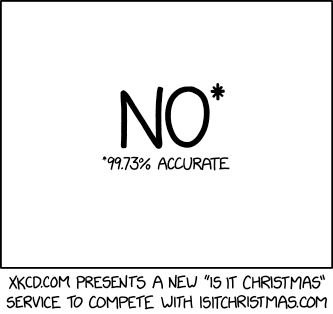
\includegraphics[height=0.6\textheight]{imgs/is_it_christmas.png}}


\begin{document}

\maketitle

\begin{frame}{Game Rules}
    \begin{minipage}{0.49\textwidth}
        \Large
        \textbf{On-Off experiment:}
        \begin{itemize}
            \item Measured $N_\text{ON}$ events in On region
            \item Measured $N_\text{OFF}$ events in Off region
            \item Time ratio $\tau$
        \end{itemize}
    \end{minipage}
    \hfill
    \begin{minipage}{0.5\textwidth}
        
\includegraphics[width=0.8\textwidth]{imgs/one_two.png}
    \end{minipage}
\end{frame}


\begin{frame}{Game Rules}
    \centering
    \Large
    \begin{align}
        &\mathcal{L}(\mu,b) = \frac{(\mu s + b)^{N_\text{ON}}}{N_\text{ON}!} e^{-(\mu s + b)} + \frac{(\tau b)^{N_\text{OFF}}}{N_\text{OFF}!} e^{-\tau b} \notag \\[4ex]
        \mu &= \text{strength parameter} \notag \\
        s &= \text{signal counts from model} \notag \\
        b &= \text{background counts from model}\notag 
    \end{align}
\end{frame}

\begin{frame}{Test statistic}
    \Large
    \centering
    \begin{align}
        q_\mu = -2 \log{\frac{\mathcal{L}(data\vert\mu,\hat{b}_\mu)}{\mathcal{L}(data\vert\hat{\mu},\hat{\hat{b})}}} \notag 
    \end{align}\\[3ex]
    $\Rightarrow$ Profiled log-likelihood ratio (pLLR)
\end{frame}

\begin{frame}{Test distribution}
    \begin{minipage}{0.49\textwidth}
        \Large
        \centering
        \begin{align}
            p = \int_{q_\mu^\text{obs}}^\infty f(q_\mu\vert \mu,\hat{b}_\mu)\,\mathcal{d}q_\mu \notag
        \end{align}
    \end{minipage}
    \hfill
    \begin{minipage}{0.5\textwidth}
        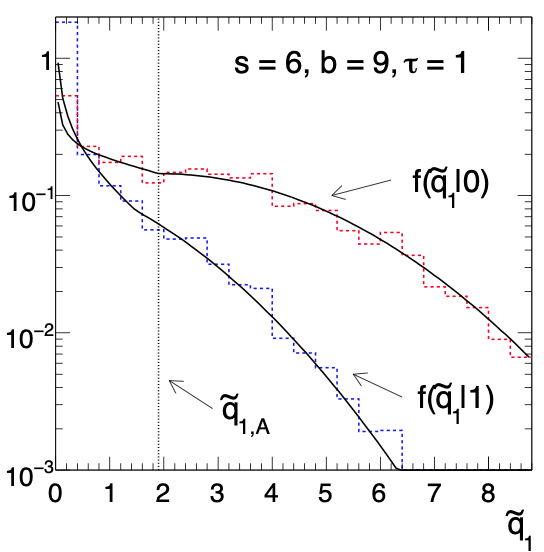
\includegraphics[width=\textwidth]{build/distribution.pdf}
    \end{minipage}
\end{frame}


\end{document}
